\documentclass[border=4pt,12pt]{standalone}
% House style for redrawn exam diagrams (diagram-v4: 0.4pt lines, filled -latex arrows, fine dashes; stipple and hatching drawn as real dots/lines (no PDF/SVG patterns, so they render in every browser and at any scale); transparent background). Every figure \input's this.
\usepackage{amsmath,amssymb}
\usepackage{txfonts}
\usepackage{pdfrender,xcolor}
% \halo{text}: label on shading. The shading stops just around each letter's outline (a thin knock-out that follows the
% glyphs, like the papers' typesetting), never a box. Owner: "I don't want a box around the text".
\newcommand{\halo}[1]{\leavevmode\rlap{\pdfrender{TextRenderingMode=2,LineWidth=2.2pt,LineJoinStyle=1,StrokeColor=white,FillColor=white}#1}#1}
\usepackage{tikz,pgfplots}
\pgfplotsset{compat=1.18}
\usetikzlibrary{arrows.meta,calc,angles,quotes,patterns,patterns.meta,intersections,positioning,decorations.markings,shapes.geometric}
% Stipple and hatching are drawn as actual dots / lines clipped to the region (path picture), NOT as pattern fills:
% SVG <pattern> fills vanish or blur when browsers scale the image, so the owner could not see the shading.
% Each dot is a 0.72pt square (keeps SVGs small; reads as a dot at print size). Dots sit on one global staggered grid, so neighbouring regions line up.
\makeatletter
\newdimen\ex@x \newdimen\ex@y \newdimen\ex@xa \newdimen\ex@ya \newdimen\ex@xb \newdimen\ex@yb \newcount\ex@row
\def\exam@stipplecolor{black!75}\def\exam@dotr{0.42pt}\def\exam@dotgap{2.5}
\def\ex@rowdots{\ifdim\ex@x<\ex@xb \pgfpathrectangle{\pgfqpoint{\dimexpr\ex@x-0.36pt\relax}{\dimexpr\ex@y-0.36pt\relax}}{\pgfqpoint{0.72pt}{0.72pt}}\advance\ex@x by \exam@dotgap pt\relax\expandafter\ex@rowdots\fi}
\def\exam@stipple{%
  \pgftransformreset% dots are sized in real points even inside scaled pictures
  \pgfpointanchor{path picture bounding box}{south west}\ex@xa=\pgf@x \ex@ya=\pgf@y
  \pgfpointanchor{path picture bounding box}{north east}\ex@xb=\pgf@x \ex@yb=\pgf@y
  \pgfsetfillcolor{\exam@stipplecolor}\pgfmathsetmacro\ex@h{\exam@dotgap/2}%
  \pgfmathtruncatemacro\ex@r{floor(\ex@ya/\ex@h)-1}\ex@row=\ex@r\relax
  \ex@y=\ex@r\dimexpr\ex@h pt\relax
  \loop\ifdim\ex@y<\ex@yb
    \pgfmathtruncatemacro\ex@c{floor(\ex@xa/\exam@dotgap)-1}\ex@x=\ex@c\dimexpr\exam@dotgap pt\relax
    \ifodd\ex@row \advance\ex@x by \ex@h pt\fi
    \ex@rowdots
    \advance\ex@y by \ex@h pt \advance\ex@row by 1
    \ifnum\numexpr\ex@row-(\ex@row/4)*4\relax=0 \pgfusepath{fill}\fi% flush every 4 rows: bounded TeX memory, few clip copies in the SVG
  \repeat\pgfusepath{fill}}
\newdimen\ex@d
\def\exam@hatch#1{% #1 = 1 for /, -1 for \ ; lines 45 degrees, 3pt apart
  \pgftransformreset
  \pgfpointanchor{path picture bounding box}{south west}\ex@xa=\pgf@x \ex@ya=\pgf@y
  \pgfpointanchor{path picture bounding box}{north east}\ex@xb=\pgf@x \ex@yb=\pgf@y
  \ex@d=\dimexpr\ex@yb-\ex@ya\relax \ex@x=\dimexpr\ex@xa-\ex@d\relax
  \loop\ifdim\ex@x<\ex@xb
    \ifnum#1>0 \pgfpathmoveto{\pgfqpoint{\ex@x}{\ex@ya}}\pgfpathlineto{\pgfqpoint{\dimexpr\ex@x+\ex@d\relax}{\ex@yb}}%
    \else \pgfpathmoveto{\pgfqpoint{\ex@x}{\ex@yb}}\pgfpathlineto{\pgfqpoint{\dimexpr\ex@x+\ex@d\relax}{\ex@ya}}\fi
    \advance\ex@x by 4.24pt
  \repeat
  \pgfsetlinewidth{0.4pt}\pgfsetstrokecolor{black}\pgfusepath{stroke}}
\def\examstipple{\exam@stipple}\def\examhatch{\exam@hatch}\def\examsetstipplecolor#1{\def\exam@stipplecolor{#1}}\def\examsetdotgap#1{\def\exam@dotgap{#1}}
\makeatother
% (legacy pattern kept for old files)
% staggered stipple like the NESA papers' dotted shading
\pgfdeclarepatternformonly{exam stipple}{\pgfpointorigin}{\pgfqpoint{2.2pt}{2.2pt}}{\pgfqpoint{2.2pt}{2.2pt}}{%
  \pgfpathcircle{\pgfqpoint{0.55pt}{0.55pt}}{0.42pt}\pgfpathcircle{\pgfqpoint{1.65pt}{1.65pt}}{0.42pt}\pgfusepath{fill}}
\tikzset{
  every picture/.style={line width=0.6pt, >={Latex[length=2mm,width=1.3mm]}},
  curve/.style={line width=0.6pt},
  open arrow/.style={-{Latex[length=2mm,width=1.3mm]}},  % owner: filled -latex heads everywhere, no open chevrons
  aux/.style={dash pattern=on 2pt off 1.5pt, line width=0.6pt},
  shade/.code={\def\exA{#1}\def\exB{none}\ifx\exA\exB\else\pgfkeysalso{fill=black!18}\fi},
  shade/.default=on,
  shade dots/.style={fill=none, path picture={\examstipple}},
  stipple color/.code={\examsetstipplecolor{#1}},
  stipple gap/.code={\examsetdotgap{#1}},
  shade dense dots/.style={fill=none, stipple gap=1.6, path picture={\examstipple}},
  shade hatch/.style={fill=none, path picture={\examhatch{1}}},
  shade hatch reverse/.style={fill=none, path picture={\examhatch{-1}}},
  shade solid/.style={fill=black},
  pt/.style={circle, fill, inner sep=1.1pt},
  open pt/.style={circle, draw, fill=white, inner sep=1.1pt},
}
\pgfplotsset{
  exam axes/.style={axis lines=middle, axis line style={->}, xlabel={$x$}, ylabel={$y$},
    xlabel style={anchor=west}, ylabel style={anchor=south}, tick label style={font=\small},
    every axis plot/.append style={line width=0.6pt, black}, samples=200, clip=false,
    enlargelimits=false, axis on top},
}

\begin{document}
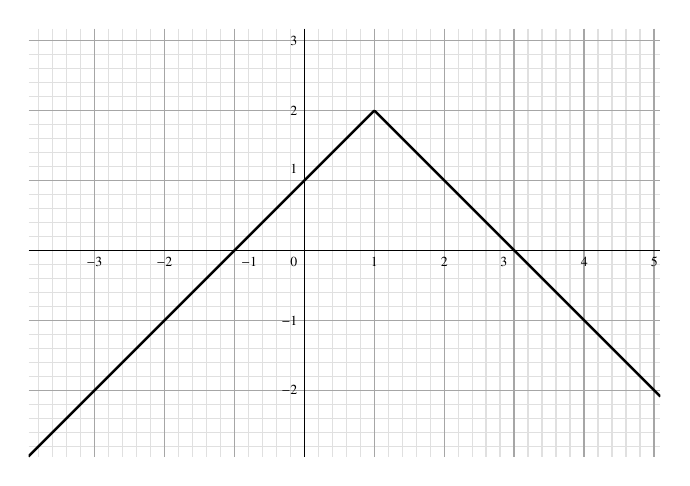
\begin{tikzpicture}[x=0.0127cm,y=-0.0127cm,font=\tiny]
\begin{scope}
\draw[black!12] (26.0,35.0) -- (26.0,464.0);
\draw[black!12] (40.0,35.0) -- (40.0,464.0);
\draw[black!12] (54.0,35.0) -- (54.0,464.0);
\draw[black!12] (68.0,35.0) -- (68.0,464.0);
\draw[black!12] (96.0,35.0) -- (96.0,464.0);
\draw[black!12] (110.0,35.0) -- (110.0,464.0);
\draw[black!12] (124.0,35.0) -- (124.0,464.0);
\draw[black!12] (138.0,35.0) -- (138.0,464.0);
\draw[black!12] (166.0,35.0) -- (166.0,464.0);
\draw[black!12] (180.0,35.0) -- (180.0,464.0);
\draw[black!12] (194.0,35.0) -- (194.0,464.0);
\draw[black!12] (208.0,35.0) -- (208.0,464.0);
\draw[black!12] (236.0,35.0) -- (236.0,464.0);
\draw[black!12] (250.0,35.0) -- (250.0,464.0);
\draw[black!12] (264.0,35.0) -- (264.0,464.0);
\draw[black!12] (278.0,35.0) -- (278.0,464.0);
\draw[black!12] (306.0,35.0) -- (306.0,464.0);
\draw[black!12] (320.0,35.0) -- (320.0,464.0);
\draw[black!12] (334.0,35.0) -- (334.0,464.0);
\draw[black!12] (348.0,35.0) -- (348.0,464.0);
\draw[black!12] (376.0,35.0) -- (376.0,464.0);
\draw[black!12] (390.0,35.0) -- (390.0,464.0);
\draw[black!12] (404.0,35.0) -- (404.0,464.0);
\draw[black!12] (418.0,35.0) -- (418.0,464.0);
\draw[black!12] (446.0,35.0) -- (446.0,464.0);
\draw[black!12] (460.0,35.0) -- (460.0,464.0);
\draw[black!12] (474.0,35.0) -- (474.0,464.0);
\draw[black!12] (488.0,35.0) -- (488.0,464.0);
\draw[black!12] (516.0,35.0) -- (516.0,464.0);
\draw[black!12] (530.0,35.0) -- (530.0,464.0);
\draw[black!12] (544.0,35.0) -- (544.0,464.0);
\draw[black!12] (558.0,35.0) -- (558.0,464.0);
\draw[black!12] (586.0,35.0) -- (586.0,464.0);
\draw[black!12] (600.0,35.0) -- (600.0,464.0);
\draw[black!12] (614.0,35.0) -- (614.0,464.0);
\draw[black!12] (628.0,35.0) -- (628.0,464.0);
\draw[black!12] (16.0,61.0) -- (648.0,61.0);
\draw[black!12] (16.0,75.0) -- (648.0,75.0);
\draw[black!12] (16.0,89.0) -- (648.0,89.0);
\draw[black!12] (16.0,103.0) -- (648.0,103.0);
\draw[black!12] (16.0,131.0) -- (648.0,131.0);
\draw[black!12] (16.0,145.0) -- (648.0,145.0);
\draw[black!12] (16.0,159.0) -- (648.0,159.0);
\draw[black!12] (16.0,173.0) -- (648.0,173.0);
\draw[black!12] (16.0,201.0) -- (648.0,201.0);
\draw[black!12] (16.0,215.0) -- (648.0,215.0);
\draw[black!12] (16.0,229.0) -- (648.0,229.0);
\draw[black!12] (16.0,243.0) -- (648.0,243.0);
\draw[black!12] (16.0,271.0) -- (648.0,271.0);
\draw[black!12] (16.0,285.0) -- (648.0,285.0);
\draw[black!12] (16.0,299.0) -- (648.0,299.0);
\draw[black!12] (16.0,313.0) -- (648.0,313.0);
\draw[black!12] (16.0,341.0) -- (648.0,341.0);
\draw[black!12] (16.0,355.0) -- (648.0,355.0);
\draw[black!12] (16.0,369.0) -- (648.0,369.0);
\draw[black!12] (16.0,383.0) -- (648.0,383.0);
\draw[black!12] (16.0,411.0) -- (648.0,411.0);
\draw[black!12] (16.0,425.0) -- (648.0,425.0);
\draw[black!12] (16.0,439.0) -- (648.0,439.0);
\draw[black!12] (16.0,453.0) -- (648.0,453.0);
\draw[black!35] (82.0,35.0) -- (82.0,464.0);
\draw[black!35] (152.0,35.0) -- (152.0,464.0);
\draw[black!35] (222.0,35.0) -- (222.0,464.0);
\draw[black!35] (362.0,35.0) -- (362.0,464.0);
\draw[black!35] (432.0,35.0) -- (432.0,464.0);
\draw[black!35] (502.0,35.0) -- (502.0,464.0);
\draw[black!35] (572.0,35.0) -- (572.0,464.0);
\draw[black!35] (642.0,35.0) -- (642.0,464.0);
\draw[black!35] (16.0,47.0) -- (648.0,47.0);
\draw[black!35] (16.0,117.0) -- (648.0,117.0);
\draw[black!35] (16.0,187.0) -- (648.0,187.0);
\draw[black!35] (16.0,327.0) -- (648.0,327.0);
\draw[black!35] (16.0,397.0) -- (648.0,397.0);
\draw (16.0,257.0) -- (648.0,257.0);
\draw (292.0,35.0) -- (292.0,464.0);
\node[anchor=north,inner sep=1.5pt] at (82.0,259.0) {$-3$};
\node[anchor=north,inner sep=1.5pt] at (152.0,259.0) {$-2$};
\node[anchor=east,inner sep=1.5pt] at (290.0,397.0) {$-2$};
\node[anchor=north west,inner sep=1.5pt] at (224.0,259.0) {$-1$};
\node[anchor=east,inner sep=1.5pt] at (290.0,327.0) {$-1$};
\node[anchor=north,inner sep=1.5pt] at (362.0,259.0) {$1$};
\node[anchor=south east,inner sep=1.5pt] at (290.0,185.0) {$1$};
\node[anchor=north,inner sep=1.5pt] at (432.0,259.0) {$2$};
\node[anchor=east,inner sep=1.5pt] at (290.0,117.0) {$2$};
\node[anchor=north east,inner sep=1.5pt] at (500.0,259.0) {$3$};
\node[anchor=east,inner sep=1.5pt] at (290.0,47.0) {$3$};
\node[anchor=north,inner sep=1.5pt] at (572.0,259.0) {$4$};
\node[anchor=north,inner sep=1.5pt] at (642.0,259.0) {$5$};
\node[anchor=north east,inner sep=1.5pt] at (290.0,259.0) {$0$};
\clip (16.0,35.0) rectangle (648.0,464.0);
\begin{scope}[shift={(292.00,257.00)},x=0.8890cm,y=0.8890cm]
\draw[line width=0.9pt] plot[domain=-3.943:5.086,samples=400] (\x,{2-abs(\x-1)});
\end{scope}
\end{scope}
\end{tikzpicture}
\end{document}
